\documentclass[11pt,a4paper]{article}
\usepackage{fontspec}
\setmainfont{Latin Modern Roman}
\usepackage{polyglossia}
\setmainlanguage{french}
\usepackage{microtype}
\usepackage[a4paper,margin=2.5cm]{geometry}
\usepackage{amsmath,amssymb}
\usepackage{graphicx}
\usepackage{booktabs}
\usepackage{xcolor}
\usepackage{caption}
\usepackage{float}
\usepackage{enumitem}
\usepackage{tikz}
\usetikzlibrary{arrows.meta,positioning}
\usepackage[hidelinks]{hyperref}

\definecolor{accent}{HTML}{C4006A}
\captionsetup{font=small,labelfont=bf,labelsep=period}
\setlist{itemsep=2pt,topsep=4pt}
\renewcommand{\arraystretch}{1.15}
\setlength{\parskip}{4pt}
\graphicspath{{figs/}}

\newcommand{\dollar}{\,\$}

\begin{document}

% ------------------------------------------------------------------ titre
\begin{titlepage}
\centering
\vspace*{3cm}
{\large Cours de Deep Learning --- GSTR, semestre 3}\\[1.2cm]
{\Huge\bfseries Agents autonomes d'investissement\\[.3cm] sur le Polkadot (DOT/USD)}\\[.8cm]
{\large Prévision par réseaux récurrents, simulation de portefeuille\\ et registre blockchain}\\[2.5cm]
{\large Tayeb Abboud}\\[.4cm]
Enseignant : C.\ Okar\\[.4cm]
Novembre 2026\\[3cm]
\begin{minipage}{.8\textwidth}\small\centering
Tout ce qui suit est de la simulation : aucun ordre n'a été passé sur un vrai marché et aucun argent réel n'est en jeu.
Le code, les données et le tableau de bord sont dans le dépôt \texttt{github.com/04MDLR80/POLKADOT\_Agent}.
\end{minipage}
\end{titlepage}

\tableofcontents
\newpage

% ------------------------------------------------------------------ 1
\section{Ce qu'on devait faire, et ce qu'on a fait}

L'énoncé demande de construire, de bout en bout, un petit système d'investissement automatisé : prévoir un prix avec un réseau
récurrent (LSTM ou GRU), confier les décisions à quatre agents autonomes (prévision, stratégie, risque, exécution), faire tourner
un portefeuille virtuel avec de vrais coûts de transaction, garder une trace infalsifiable des décisions dans une chaîne de blocs que
l'enseignant peut vérifier, puis présenter le tout dans un tableau de bord et un rapport.

L'énoncé parle de l'or. Nous avons travaillé sur le Polkadot (DOT) à la place, avec l'accord de l'enseignant. Ce choix a un coût :
le DOT est bien plus agité que l'or, et nous y reviendrons souvent, car il explique une bonne partie de nos résultats. Il a aussi un avantage
pratique : son marché est ouvert en continu et ses prix sont disponibles par une API publique, ce qui nous a permis d'ajouter une simulation
en direct (section~\ref{sec:direct}).

Voici, en une page, ce que nous avons obtenu.

\begin{itemize}
\item Un jeu de 2\,096 jours de prix du DOT en dollars, du 8 février 2021 au 4 novembre 2026, nettoyé et analysé (section~\ref{sec:donnees}).
\item Deux réseaux écrits à la main en NumPy, un LSTM et un GRU, avec leurs gradients vérifiés numériquement (section~\ref{sec:modeles}).
Le LSTM a été retenu sur la validation.
\item Quatre agents, un moteur de portefeuille avec frais et glissement, et un protocole qui interdit toute fuite d'information
(sections~\ref{sec:agents} et~\ref{sec:protocole}).
\item Un registre SHA-256 chaîné, avec preuve de travail légère et vérification complète (section~\ref{sec:chaine}).
\item Un résultat à lire avec prudence : sur la période de test, les agents finissent à $-18{,}1\,\%$ alors que garder le DOT aurait fait
$-75{,}3\,\%$. Mais nos réseaux ne prévoient pas mieux qu'une prévision naïve, et l'écart vient surtout du coupe-circuit de l'agent de
risque (section~\ref{sec:resultats}).
\item Un tableau de bord Streamlit et des agents qui tournent seuls tous les jours sur GitHub (section~\ref{sec:direct}).
\end{itemize}

\begin{figure}[H]\centering
\begin{tikzpicture}[node distance=7mm,>=Stealth,
  b/.style={draw=black!60,rounded corners=2pt,minimum height=9mm,minimum width=22mm,align=center,font=\footnotesize,fill=white}]
\node[b] (d) {Prix\\quotidiens};
\node[b,right=of d] (p) {Variables\\fenêtres};
\node[b,right=of p] (r) {LSTM / GRU\\(5 réseaux)};
\node[b,right=of r,fill=accent!12] (a) {Agents\\stratégie, risque};
\node[b,right=of a] (e) {Exécution\\portefeuille};
\draw[->] (d)--(p); \draw[->] (p)--(r); \draw[->] (r)--(a); \draw[->] (a)--(e);
\node[b,below=8mm of a,minimum width=100mm] (c) {Registre blockchain : un bloc par agent et par jour};
\foreach \n in {r,a,e} \draw[->,black!45] (\n.south) -- (\n.south |- c.north);
\end{tikzpicture}
\caption{Vue d'ensemble du système.}
\end{figure}

% ------------------------------------------------------------------ 2
\section{Les données}\label{sec:donnees}

\subsection{D'où elles viennent}

Nous avons téléchargé l'historique complet du DOT/USD sur Investing.com : ouverture, plus haut, plus bas, clôture et volume, un point par jour.
Le fichier compte 2\,096 jours, du 8 février 2021 au 4 novembre 2026. Un seul jour manque, le 12 janvier 2025. Nous l'avons comblé avec la
clôture de la veille (rendement nul ce jour-là) plutôt que de supprimer la ligne, pour ne pas décaler les fenêtres de 20 jours qui suivent.
Les volumes, écrits avec des suffixes K, M ou B, ont été convertis en nombres.

\subsection{Un actif très agité qui a beaucoup baissé}

Le prix passe de 23,01\dollar{} au départ à 0,93\dollar{} à la fin. Le sommet est à 53,84\dollar{} (4 novembre 2021) et le plancher à 0,75\dollar{}
(18 août 2026), soit une perte de 98,6\,\% depuis le sommet. La volatilité annualisée est d'environ 93\,\%. Le tableau~\ref{tab:annees} montre
que le régime change beaucoup d'une année à l'autre : un rebond de $+91\,\%$ en 2023 entre deux années de chute.

\begin{table}[H]\centering\small
\begin{tabular}{rrrr}\toprule
Année & Rendement & Volatilité annualisée & Jours \\\midrule
2021 & +16\,\% & 139\,\% & 327 \\
2022 & $-$84\,\% & 94\,\% & 365 \\
2023 & +91\,\% & 64\,\% & 365 \\
2024 & $-$19\,\% & 84\,\% & 366 \\
2025 & $-$73\,\% & 86\,\% & 365 \\
2026 & $-$48\,\% & 79\,\% & 308 \\
\bottomrule\end{tabular}

\caption{Rendement et volatilité du DOT par année (2021 et 2026 sont incomplètes).}\label{tab:annees}
\end{table}

\begin{figure}[H]\centering
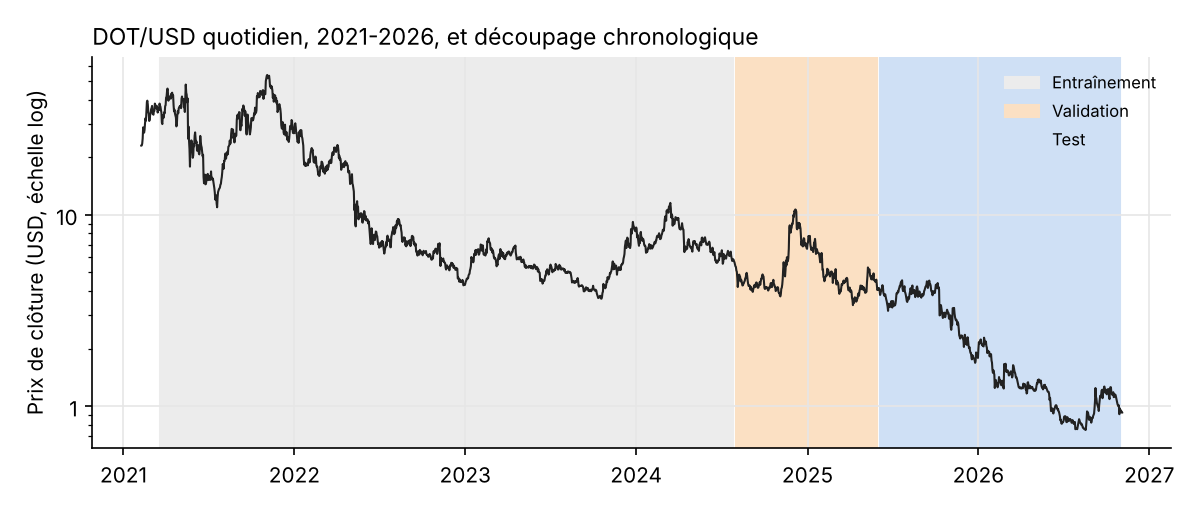
\includegraphics[width=.92\textwidth]{fig1_prix.png}
\caption{Prix de clôture du DOT/USD.}
\end{figure}

Quelques résultats de l'analyse exploratoire comptent pour la suite.

\begin{itemize}
\item \textbf{Le prix n'est pas stationnaire.} Le test de Dickey-Fuller augmenté sur le logarithme du prix donne $-0{,}70$, loin de la valeur
critique à 5\,\% ($-2{,}86$). Sur les rendements, il donne $-33{,}5$ : les rendements sont stationnaires. C'est pourquoi nous prévoyons des
rendements et non des prix.
\item \textbf{Les rendements ont des queues très lourdes.} Le kurtosis en excès est de 8,6 et le test de Jarque-Bera rejette la normalité
(statistique 6\,514). Le pire jour vaut $-0{,}485$ en rendement logarithmique (19 mai 2021).
\item \textbf{Presque aucune mémoire dans le sens des rendements, mais une forte mémoire dans leur amplitude.} L'autocorrélation à un jour est de
$-0{,}024$. Le test de Ljung-Box sur les rendements est à peine significatif (statistique 26, $p=0{,}004$), alors que sur les rendements au carré
il est écrasant (274, $p<10^{-3}$) : les périodes calmes et agitées se regroupent, mais le signe du rendement de demain n'est pas écrit dans celui d'hier.
\end{itemize}

Ce dernier point donne le ton : un réseau peut apprendre quand la volatilité monte, beaucoup moins dans quel sens le prix va partir.

\begin{figure}[H]\centering
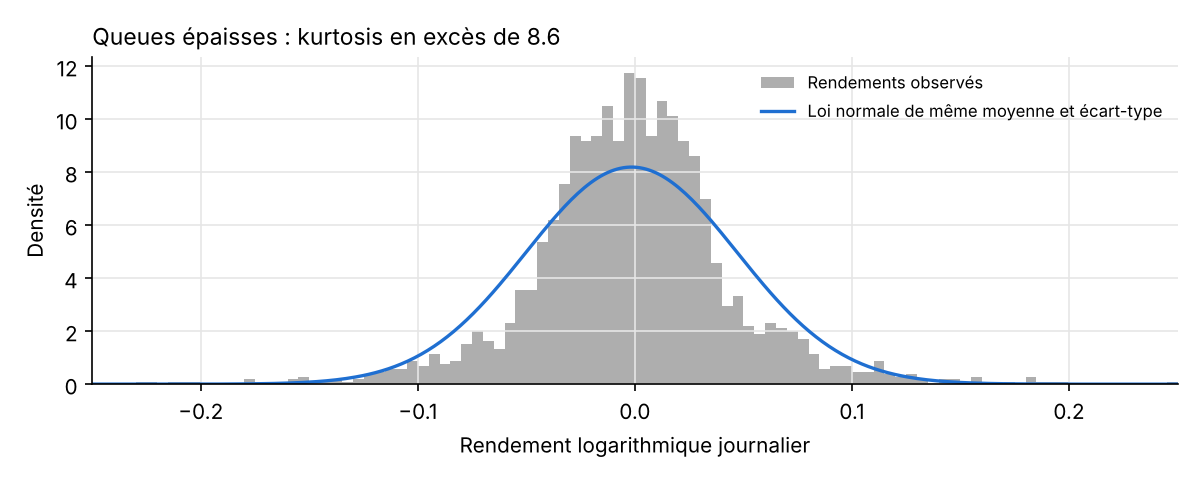
\includegraphics[width=.48\textwidth]{fig2_distribution.png}\hfill
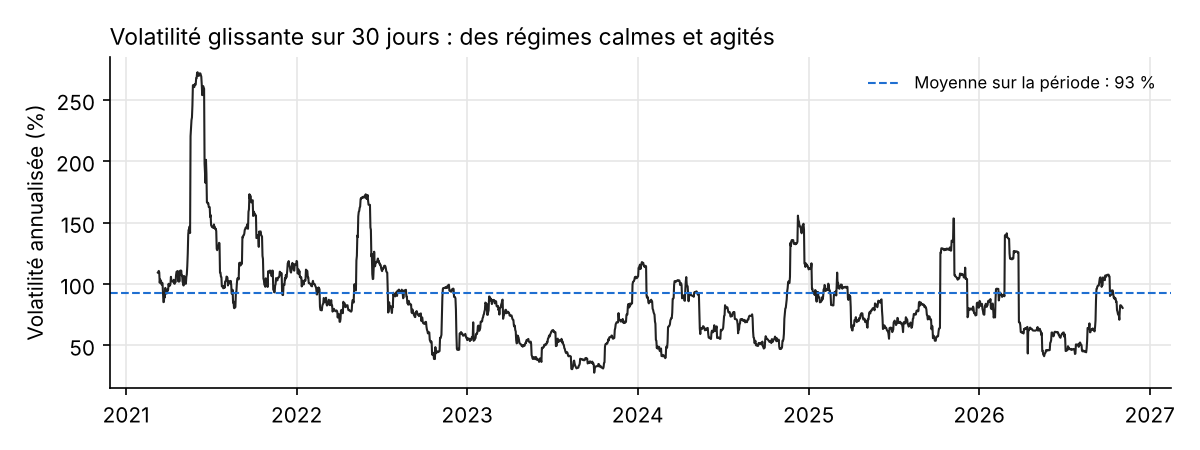
\includegraphics[width=.48\textwidth]{fig3_volatilite.png}
\caption{À gauche, distribution des rendements journaliers comparée à une loi normale. À droite, volatilité glissante.}
\end{figure}

\begin{figure}[H]\centering
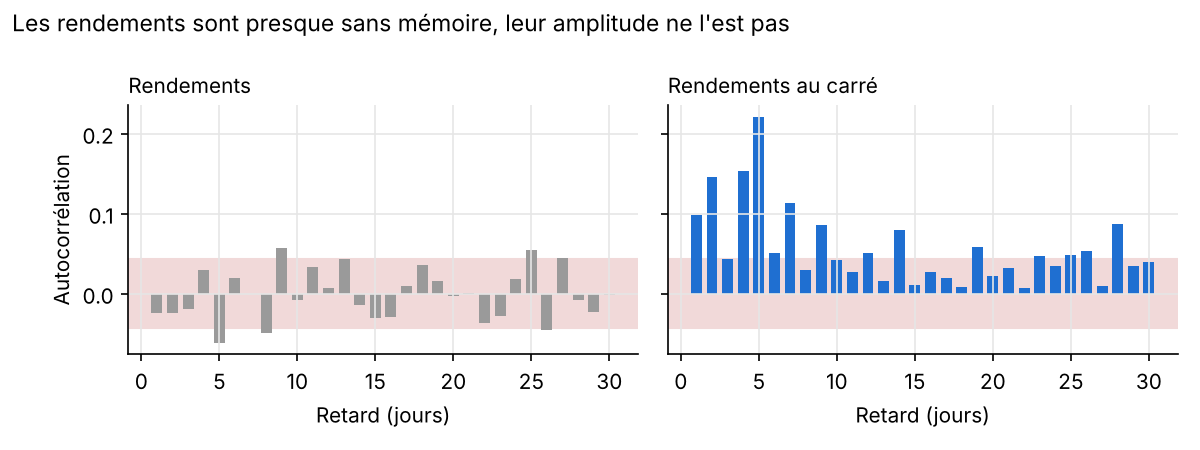
\includegraphics[width=.8\textwidth]{fig4_acf.png}
\caption{Autocorrélation des rendements et des rendements au carré.}
\end{figure}

% ------------------------------------------------------------------ 3
\section{Préparer les données pour le réseau}\label{sec:prep}

\subsection{Variables et cible}

À chaque jour $t$, nous calculons huit variables à partir de ce qui est connu à la clôture : le rendement logarithmique, l'amplitude
$(H-L)/C$, la variation du volume, l'écart de la clôture à sa moyenne mobile sur 20 jours, le momentum sur 5 et 20 jours, la volatilité sur
20 jours et le RSI sur 14 jours. Chaque exemple est une fenêtre des 20 derniers jours de ces huit variables.

La cible est le rendement logarithmique cumulé sur les cinq jours suivants :
\[
y_t=\ln\frac{C_{t+5}}{C_t}.
\]

Nous avions commencé par prévoir le rendement du lendemain. C'était une impasse : les prévisions étaient toutes plus petites que le coût d'un
aller-retour (0,62\,\%), donc la stratégie ne passait aucun ordre. Un horizon de cinq jours laisse au signal le temps de dépasser les frais, et il est
plus simple à prévoir parce que le bruit d'un seul jour pèse moins. Nous avons aussi enrichi les variables (momentum, volatilité, RSI) à ce moment-là.

\subsection{Découpage sans fuite}

Le découpage est chronologique : 60\,\% pour l'entraînement (1\,226 fenêtres), 15\,\% pour la validation (303) et 25\,\% pour le test (513).
Le test couvre du 5 juin 2025 au 31 octobre 2026. Comme la cible regarde cinq jours devant, une fenêtre située juste avant une frontière contient en
partie le futur de l'ensemble suivant. Nous retirons donc cinq fenêtres de chaque côté des frontières (purge). La moyenne et l'écart-type servant à
normaliser les variables sont calculés sur l'entraînement seul, puis appliqués tels quels à la validation et au test.

% ------------------------------------------------------------------ 4
\section{Les réseaux}\label{sec:modeles}

\subsection{Pourquoi les avoir écrits nous-mêmes}

PyTorch et TensorFlow n'étaient pas installables dans notre environnement de travail. Plutôt que de renoncer, nous avons codé le GRU et le LSTM en
NumPy, avec la rétropropagation à travers le temps écrite à la main. Cela nous a obligés à comprendre chaque porte, et cela a un prix : des
réseaux petits, entraînés sur CPU.

\subsection{Les équations}

Le GRU, pour une entrée $x_t$ et un état caché $h_{t-1}$ :
\begin{align*}
z_t&=\sigma(W_z x_t+U_z h_{t-1}+b_z), & r_t&=\sigma(W_r x_t+U_r h_{t-1}+b_r),\\
\tilde h_t&=\tanh\big(W_n x_t+U_n(r_t\odot h_{t-1})+b_n\big), & h_t&=(1-z_t)\odot\tilde h_t+z_t\odot h_{t-1}.
\end{align*}

Le LSTM ajoute une cellule mémoire $c_t$ et trois portes (entrée $i$, oubli $f$, sortie $o$) :
\begin{align*}
i_t,f_t,o_t&=\sigma(W_\bullet x_t+U_\bullet h_{t-1}+b_\bullet), & g_t&=\tanh(W_g x_t+U_g h_{t-1}+b_g),\\
c_t&=f_t\odot c_{t-1}+i_t\odot g_t, & h_t&=o_t\odot\tanh(c_t).
\end{align*}
Le biais de la porte d'oubli est initialisé à 1 pour que la cellule garde l'information par défaut. Dans les deux cas, une couche linéaire lit le dernier
état caché $h_{20}$ et produit le rendement prévu (normalisé).

\subsection{Vérifier que le gradient est juste}

Un gradient faux ne plante pas, il entraîne simplement mal. Nous avons donc comparé le gradient analytique à une différence finie centrée sur des
paramètres tirés au hasard. L'erreur relative maximale est de $4\times10^{-7}$ pour le LSTM et de $8\times10^{-7}$ pour le GRU, ce qui valide
l'implémentation.

\subsection{Entraînement et choix du modèle}

L'entraînement utilise l'optimiseur Adam (pas 0,01), un écrêtage du gradient à 1, une pénalité L2 et un arrêt anticipé : on garde les poids qui ont la
plus petite erreur de validation, et on arrête après 80 époques sans amélioration (600 au maximum). Nous entraînons cinq réseaux avec des
initialisations différentes. La moyenne de leurs prévisions est le rendement prévu $\mu$, et leur écart-type mesure l'incertitude $\sigma$, que les agents
utiliseront. Les LSTM se sont arrêtés entre 122 et 214 époques.

\begin{table}[H]\centering\small
\begin{tabular}{lrrr}\toprule
Famille & Unités cachées & Pénalité L2 & RMSE de validation \\\midrule
GRU & 4 & 0,01 & 0,1071 \\
GRU & 8 & 0,01 & 0,1078 \\
GRU & 8 & 0,001 & 0,1062 \\
LSTM & 4 & 0,01 & 0,1036 \\
LSTM & 8 & 0,01 & 0,1044 \\
LSTM & 8 & 0,001 & 0,1047 \\
\bottomrule\end{tabular}

\caption{Recherche d'hyperparamètres, mesurée sur la validation seulement.}\label{tab:hyper}
\end{table}

Le meilleur réglage est un LSTM à 4 unités avec $\lambda=0{,}01$ (RMSE de validation 0,1036), devant le meilleur GRU (0,1062). Les écarts entre les réglages sont petits.
Les petits réseaux gagnent : avec 1\,226 exemples d'entraînement et un signal aussi faible, un réseau plus gros apprend surtout le bruit.

\begin{figure}[H]\centering
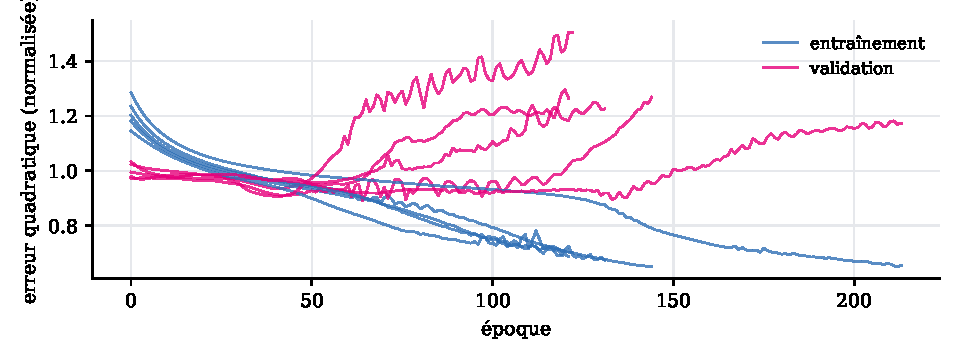
\includegraphics[width=.85\textwidth]{apprentissage.pdf}
\caption{Erreur d'entraînement et de validation des cinq LSTM. La validation remonte après quelques dizaines d'époques : c'est le signe du surapprentissage que l'arrêt anticipé évite.}
\end{figure}

% ------------------------------------------------------------------ 5
\section{Les quatre agents}\label{sec:agents}

Chaque agent a un rôle étroit et ne connaît que ce que lui transmet le précédent.

\begin{enumerate}
\item \textbf{Agent de prévision.} Il fait tourner l'ensemble de réseaux sur les 20 derniers jours et renvoie $\mu$ et $\sigma$.
\item \textbf{Agent de stratégie.} Il achète si $\mu>0{,}62\,\%$ \emph{et} $\mu>0{,}5\,\sigma$. Il vend si $\mu<-0{,}56\,\%$. Sinon il conserve.
Le seuil d'achat est le coût d'un aller-retour, $2\times(0{,}26\,\%+0{,}05\,\%)$ : en dessous, un trade perd de l'argent même si la prévision est juste.
Le seuil de vente est le 40\textsuperscript{e} centile des prévisions de validation, donc fixé sans regarder le test. La deuxième condition
d'achat évite d'agir quand les cinq réseaux se contredisent.
\item \textbf{Agent de risque.} Il peut modifier ou refuser l'ordre : exposition maximale de 80\,\% du portefeuille, stop-loss à $-10\,\%$ du prix d'entrée,
ordre minimal de 50\dollar{}, et coupe-circuit qui interdit tout achat quand la valeur du portefeuille descend sous 85\,\% du capital initial.
\item \textbf{Agent d'exécution.} Il passe l'ordre au prix d'ouverture du lendemain, avec 0,26\,\% de frais et 0,05\,\% de glissement,
et met à jour la trésorerie et la position.
\end{enumerate}

% ------------------------------------------------------------------ 6
\section{Le protocole de simulation}\label{sec:protocole}

Le point le plus délicat d'un backtest est la fuite d'information. Notre règle est simple : la décision du jour $t$ n'utilise que les données jusqu'à la
\emph{clôture} de $t$, et l'ordre est exécuté à l'\emph{ouverture} de $t+1$. Le portefeuille démarre à 10\,000\dollar{} le 5 juin 2025 et est valorisé
chaque jour à la clôture. Nous comparons les agents à garder le DOT sans rien faire (Buy and Hold), une règle technique
(acheter quand la clôture passe au-dessus de sa moyenne sur 20 jours, vendre sinon) et à deux prévisions naïves (zéro, et la moyenne du rendement
sur l'entraînement).

% ------------------------------------------------------------------ 7
\section{La chaîne de blocs}\label{sec:chaine}

Chaque jour, chacun des quatre agents ajoute un bloc contenant sa décision et ses paramètres. Un bloc porte l'empreinte SHA-256 du bloc précédent,
un compteur (nonce) choisi pour que sa propre empreinte commence par trois zéros (preuve de travail légère), et l'horodatage. Si quelqu'un modifie
une décision passée, l'empreinte de ce bloc change, donc celle du suivant ne correspond plus, et ainsi de suite jusqu'au bout : la vérification
détecte l'altération. Le registre de la période de test compte 2\,055 blocs et passe la vérification. Nous avons aussi essayé de le falsifier
à la main en modifiant des blocs : le contrôle l'a refusé chaque fois. Le fichier \texttt{ledger.json}
et le script \texttt{verify\_chain.py} permettent à l'enseignant de refaire la vérification.

% ------------------------------------------------------------------ 8
\section{Résultats}\label{sec:resultats}

\subsection{Les réseaux prévoient-ils mieux qu'une règle triviale ?}

Pas sur le test. Le tableau~\ref{tab:prev} compare les erreurs de prévision du rendement à cinq jours.

\begin{table}[H]\centering\small
\begin{tabular}{lrrrrrr}\toprule
 & \multicolumn{3}{c}{Validation} & \multicolumn{3}{c}{Test} \\\cmidrule(lr){2-4}\cmidrule(lr){5-7}
Modèle & MAE & RMSE & Direction & MAE & RMSE & Direction \\\midrule
LSTM & 0,0791 & 0,1036 & 58\,\% & 0,0698 & 0,0914 & 53\,\% \\
GRU & 0,0803 & 0,1062 & 53\,\% & 0,0696 & 0,0919 & 51\,\% \\
Prévision nulle & 0,0821 & 0,1083 & -- & 0,0696 & 0,0896 & -- \\
Moyenne du train & 0,0821 & 0,1083 & 52\,\% & 0,0684 & 0,0887 & 59\,\% \\
\bottomrule\end{tabular}

\caption{Erreur de prévision. « Direction » est la part des jours où le signe prévu est le bon.}\label{tab:prev}
\end{table}

Sur la validation, le LSTM (RMSE 0,1036) fait mieux que les deux références (0,1083). C'est ce qui nous a fait le choisir. Sur le test, la situation s'inverse :
la moyenne du train donne 0,0887, le LSTM 0,0914 et le GRU 0,0919. La prévision de la direction est à peu près un pile ou face (53\,\% pour le LSTM).
La moyenne du train «~réussit~» mieux (59\,\%) pour une raison sans intérêt : elle est négative, et le DOT a surtout baissé pendant le test.
Notre lecture est que le modèle a retenu des régularités de la période 2021--2024 qui ne tiennent plus en 2025--2026, et qu'il n'y a de toute façon pas
beaucoup de signal à extraire de ces variables.

\begin{figure}[H]\centering
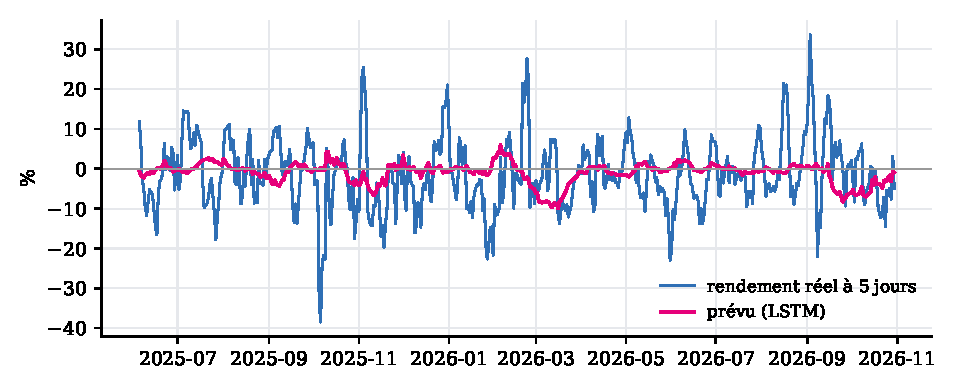
\includegraphics[width=.92\textwidth]{previsions.pdf}
\caption{Rendement à cinq jours réel et prévu par le LSTM sur le test. Les prévisions restent dans une bande étroite autour de zéro.}
\end{figure}

\subsection{Le portefeuille}

\begin{table}[H]\centering\small
\begin{tabular}{lrrrrr}\toprule
Stratégie & Valeur finale (\$) & Rendement & Drawdown max & Sharpe & Ordres \\\midrule
Agents LSTM (retenu) & 8\,187 & $-$18,1\,\% & $-$29,2\,\% & $-$0,56 & 16 \\
Agents GRU & 8\,415 & $-$15,8\,\% & $-$23,3\,\% & $-$0,57 & 17 \\
Règle technique MM20 & 8\,097 & $-$19,0\,\% & $-$30,4\,\% & $-$0,84 & 15 \\
Buy and Hold & 2\,469 & $-$75,3\,\% & $-$83,5\,\% & $-$0,78 & 1 \\
Agents LSTM sans coupe-circuit & 6\,311 & $-$36,9\,\% & $-$54,6\,\% & $-$0,70 & 45 \\
\bottomrule\end{tabular}

\caption{Résultats sur le test (513 jours, capital initial 10\,000\dollar{}).}\label{tab:strat}
\end{table}

\begin{figure}[H]\centering
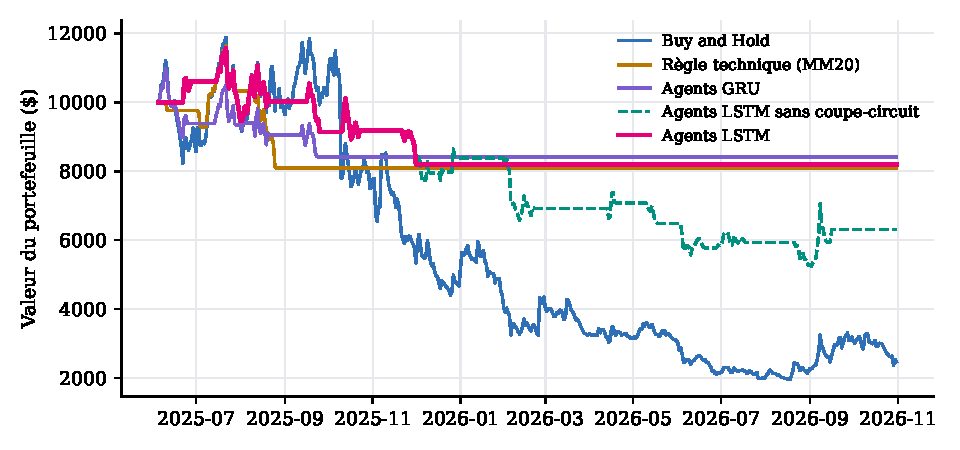
\includegraphics[width=.92\textwidth]{valeur.pdf}
\caption{Valeur du portefeuille sur la période de test.}
\end{figure}

Les agents terminent à 8\,187\dollar{} ($-18{,}1\,\%$), contre 2\,469\dollar{} pour le Buy and Hold ($-75{,}3\,\%$) : la différence est énorme, mais elle ne
vient pas d'une bonne prévision. Il faut regarder ce qui s'est passé jour par jour.

\begin{figure}[H]\centering
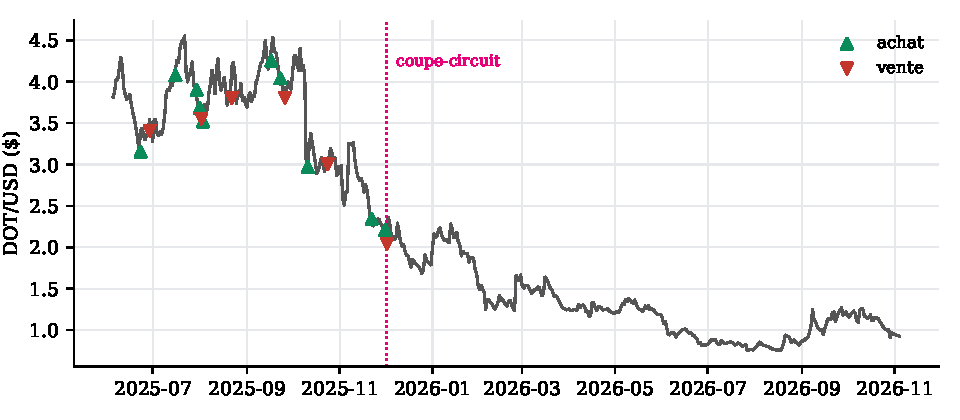
\includegraphics[width=.92\textwidth]{ordres.pdf}
\caption{Prix du DOT sur le test, achats et ventes des agents.}
\end{figure}

\begin{table}[H]\centering\small
\begin{tabular}{lrrl}\toprule
Date d'exécution & Ordre & Prix (\$) & Motif \\\midrule
23/06/2025 & acheter & 3,155 & achat validé \\
29/06/2025 & vendre & 3,408 & signal de vente \\
16/07/2025 & acheter & 4,079 & achat validé \\
30/07/2025 & acheter & 3,903 & achat validé \\
01/08/2025 & acheter & 3,688 & achat validé \\
02/08/2025 & vendre & 3,554 & stop-loss \\
03/08/2025 & acheter & 3,520 & achat validé \\
22/08/2025 & vendre & 3,801 & signal de vente \\
17/09/2025 & acheter & 4,252 & achat validé \\
23/09/2025 & acheter & 4,040 & achat validé \\
26/09/2025 & vendre & 3,804 & stop-loss \\
11/10/2025 & acheter & 2,969 & achat validé \\
24/10/2025 & vendre & 3,003 & signal de vente \\
22/11/2025 & acheter & 2,347 & achat validé \\
01/12/2025 & acheter & 2,208 & achat validé \\
02/12/2025 & vendre & 2,043 & stop-loss \\
\bottomrule\end{tabular}

\caption{Les 16 ordres du LSTM.}
\end{table}

Après le stop-loss du 2 décembre 2025, le portefeuille vaut 8\,187\dollar{}, sous le seuil de 8\,500\dollar{} (85\,\% du capital). Le coupe-circuit interdit alors
tout nouvel achat, et les agents restent en dollars jusqu'à la fin pendant que le DOT continue de chuter. Sans coupe-circuit (ligne en pointillés),
les agents rachètent la baisse, se font stopper plusieurs fois et finissent à 6\,311\dollar{} ($-36{,}9\,\%$) avec 45 ordres. Autrement dit, \emph{le gain
vient de l'interdiction d'acheter, pas de la capacité à prévoir}. La règle technique MM20, sans aucun réseau, finit à 8\,097\dollar{}, dans le même ordre
de grandeur. Le GRU (8\,415\dollar{}) fait un peu mieux que le LSTM, mais l'écart est dans le bruit : nous n'avons pas de quoi dire qu'un réseau est
meilleur que l'autre sur le test.

\subsection{Sensibilité aux paramètres}

\begin{table}[H]\centering\small
\begin{tabular}{llrrr}\toprule
Paramètre & Valeur & Valeur finale (\$) & Rendement & Drawdown max \\\midrule
Référence & - & 8\,187 & $-$18,1\,\% & $-$29,2\,\% \\
Coupe-circuit & aucun & 6\,311 & $-$36,9\,\% & $-$54,6\,\% \\
Coupe-circuit & 75 \,\% & 7\,044 & $-$29,6\,\% & $-$39,1\,\% \\
Coupe-circuit & 90 \,\% & 8\,907 & $-$10,9\,\% & $-$23,0\,\% \\
Stop-loss & aucun & 8\,339 & $-$16,6\,\% & $-$27,9\,\% \\
Stop-loss & 5 \,\% & 8\,396 & $-$16,0\,\% & $-$27,4\,\% \\
Stop-loss & 20 \,\% & 8\,339 & $-$16,6\,\% & $-$27,9\,\% \\
Plafond d'exposition & 50 \,\% & 8\,076 & $-$19,2\,\% & $-$26,3\,\% \\
Plafond d'exposition & 100 \,\% & 8\,380 & $-$16,2\,\% & $-$30,0\,\% \\
Frais par ordre & 0,10 \,\% & 8\,315 & $-$16,8\,\% & $-$28,3\,\% \\
Frais par ordre & 0,50 \,\% & 8\,004 & $-$20,0\,\% & $-$30,4\,\% \\
Seuil d'achat & 0,30 \,\% & 8\,296 & $-$17,0\,\% & $-$29,7\,\% \\
Seuil d'achat & 1,50 \,\% & 7\,997 & $-$20,0\,\% & $-$29,7\,\% \\
\bottomrule\end{tabular}

\caption{Un paramètre change à la fois, les autres restent à leur valeur de référence.}\label{tab:sensi}
\end{table}

Le tableau~\ref{tab:sensi} confirme que les paramètres de risque pèsent plus que la prévision. Le niveau du coupe-circuit fait passer le résultat de
$-10{,}9\,\%$ (seuil à 90\,\%) à $-36{,}9\,\%$ (pas de coupe-circuit). Le stop-loss, le plafond d'exposition, les frais et le seuil d'achat changent le
résultat de quelques points seulement. Nous avons fixé ces paramètres avant de voir le test et nous ne les avons pas ajustés ensuite : choisir celui qui donne
$-10{,}9\,\%$ serait du sur-ajustement sur le test.

% ------------------------------------------------------------------ 9
\section{Du backtest à la simulation en direct}\label{sec:direct}

Une fois le backtest terminé, nous avons voulu voir les agents travailler en vrai. Le modèle entraîné est sauvegardé (\texttt{modele\_live.npz}) et rechargé
par un programme qui lit le prix du DOT/USD sur l'API publique de Kraken, sans compte ni clé. Les agents prennent une décision par jour, juste après la
clôture de 00:00 UTC, car le modèle a été entraîné sur des bougies quotidiennes. Le prix est lu plus souvent pour valoriser le portefeuille.

Pour que tout tourne sans intervention, un workflow GitHub Actions se lance à 00:05 UTC puis toutes les quatre heures. Il récupère les prix, fait décider les
agents s'il y a une nouvelle bougie clôturée, ajoute les blocs au registre et enregistre l'état dans le dépôt. Le tableau de bord Streamlit lit cet état et
se met à jour à chaque enregistrement. Au premier passage, le 7 novembre 2026, les agents ont prévu $-0{,}93\,\%$ sur cinq jours à partir de la dernière
clôture et sont restés en dollars. Quelques jours de fonctionnement ne disent rien de la qualité de la stratégie : un résultat sur une semaine n'a pas de valeur statistique.

% ------------------------------------------------------------------ 10
\section{Limites et suite}\label{sec:limites}

\begin{itemize}
\item \textbf{Pas de pouvoir prédictif démontré.} Sur le test, le modèle ne bat pas une prévision triviale. Nous l'avons écrit tel quel plutôt que de chercher un
réglage qui aurait donné un meilleur chiffre.
\item \textbf{Un seul actif, un seul test.} Le test est une unique trajectoire, très baissière. Une autre période, ou une validation glissante (walk-forward),
donnerait une image plus solide.
\item \textbf{Peu de données pour du Deep Learning.} 1\,226 exemples d'entraînement, c'est peu. Des données horaires, ou plusieurs actifs, aideraient.
\item \textbf{Un modèle de coûts simple.} Frais et glissement fixes ; pas d'impact sur le prix, pas d'ordres partiels.
\item \textbf{Une blockchain pédagogique.} Une seule machine écrit le registre : il garantit l'intégrité de l'historique, pas la décentralisation.
\end{itemize}

Ce que nous ferions ensuite : une validation par fenêtres glissantes, des variables d'un autre type (flux sur la chaîne, indice de peur et d'avidité),
et une prévision de la volatilité, que nos tests statistiques montrent bien plus prévisible que le signe du rendement.

% ------------------------------------------------------------------ 11
\section{Conclusion}

Nous avons construit un système complet et honnête : des données propres, deux réseaux dont les gradients sont vérifiés, quatre agents, un protocole sans fuite
d'information, un registre vérifiable, un tableau de bord et une simulation en direct. Le résultat financier est meilleur que celui du Buy and Hold, mais ce
n'est pas grâce à la prévision : c'est le coupe-circuit qui a évité d'acheter une chute de $-75\,\%$. Si nous devions retenir une leçon, ce serait celle-là :
sur un actif aussi bruité, la gestion du risque compte plus que le modèle, et un bon protocole d'évaluation sert surtout à ne pas se raconter d'histoires.

\appendix
\section{Livrables et reproduction}

\begin{itemize}
\item Dépôt : \texttt{github.com/04MDLR80/POLKADOT\_Agent}.
\item \texttt{python3 main.py data/dot\_usd\_complet.csv} : entraîne les réseaux et lance les simulations (environ 2 minutes).
\item \texttt{python3 verify\_chain.py outputs/ledger.json} : vérifie le registre.
\item \texttt{streamlit run streamlit\_app.py} : tableau de bord.
\item \texttt{python3 trade\_daily.py} : un passage des agents en direct (appelé par GitHub Actions).
\item \texttt{python3 rapport/assets.py} puis \texttt{latexmk -pdf rapport/rapport.tex} : régénère les figures, les tableaux et ce rapport.
\end{itemize}

Données : Investing.com (DOT/USD historique) et API publique de Kraken pour le direct.

\end{document}
